\documentclass{article}

\usepackage{report/context/arxiv}

\usepackage[utf8]{inputenc} % allow utf-8 input
\usepackage[T1]{fontenc}    % use 8-bit T1 fonts
\usepackage{amsmath}
\usepackage{hyperref}       % hyperlinks
\usepackage{url}            % simple URL typesetting
\usepackage{booktabs}       % professional-quality tables
\usepackage{amsfonts}       % blackboard math symbols
% \usepackage{nicefrac}       % compact symbols for 1/2, etc.
% \usepackage{microtype}      % microtypography
% \usepackage{lipsum}		% Can be removed after putting your text content
\usepackage{graphicx}
\usepackage{natbib}
% \usepackage{doi}
\usepackage{float}
\usepackage{subcaption}


\title{[TITLE]}


\author{ \href{https://orcid.org/0000-0000-0000-0000}{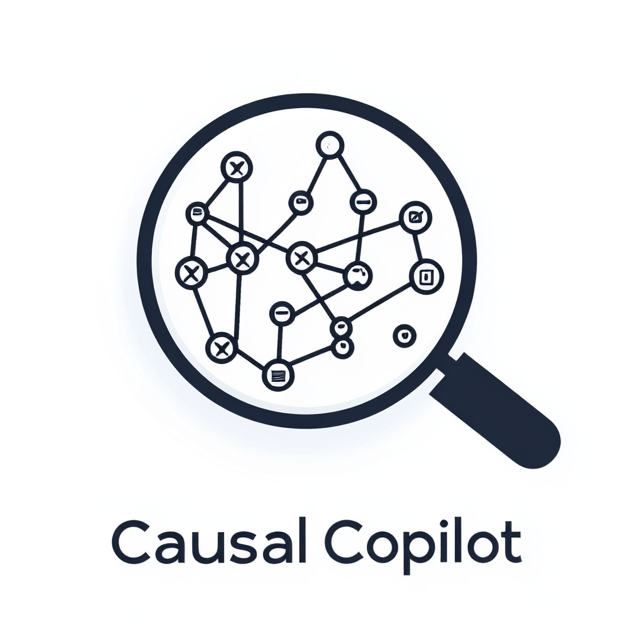
\includegraphics[scale=0.06]{asset/logo.png}} }
	

\renewcommand{\headeright}{Technical Report}
\renewcommand{\undertitle}{Technical Report}

\hypersetup{
pdftitle={[TITLE]},
pdfauthor={Causal Copilot},
pdfkeywords={Causal Discovery, Large Language Model, [ALGO]},
}

\begin{document}
\maketitle

\begin{abstract}
[ABSTRACT]
\end{abstract}

\keywords{Causal Discovery, Large Language Model, [ALGO]}

\raggedbottom
\section{Introduction}
[INTRO_INFO]

\section{Dataset Descriptions and EDA}
The following is a preview of our original dataset. Please note that if the column number is greater than 20,
we randomly choose 20 columns to be shown there.

\begin{table}[H]
    \centering
    \caption{Dataset Preview}
    [DATA_PREVIEW]
\end{table}

\subsection{Data Properties}
We employ several statistical methods to identify data properties.

The shape of the data, data types, and missing values are assessed directly from the dataframe, and Time-Series and Heterogeneity are derived from user queries.

We conducted the Ramsey's RESET test to assess linearity between each pair of variables, provided the total number of tests was fewer than 100. If the number of tests exceeded 100, we randomly selected 100 variable pairs for testing.
To correct for multiple testing, we applied the Benjamini and Yekutieli procedure, which is robust when dealing with dependent or correlated data. 
The linearity assumption was considered satisfied if all tested variable pairs demonstrated linearity; otherwise, it was considered violated if at least one pair showed non-linearity.

The assumption of Gaussian noise was tested using the Shapiro-Wilk test. The testing procedures were similar to those for linearity and depended on the concluded linearity assumption. 
If the dataset was found to satisfy the linearity assumption, we fitted an OLS model between each pair of variables and obtained the residuals. 
If the dataset did not satisfy the linearity assumption, we employed a flexible non-parametric method, locally weighted scatterplot smoothing (LOWESS), to fit the model and obtain the residuals. 
Again, we used the Benjamini and Yekutieli procedure to correct for multiple testing results. 

[PREPROCESS_GRAPH]


Properties of the dataset we analyzed are listed below.

\begin{table}[H]
    \centering
    \caption{Data Properties}
[DATA_PROP_TABLE]
\end{table}


\subsection{Distribution Analysis}
The following figure shows distributions of different variables. The orange dash line represents the mean, 
and the black line represents the median. Variables are categorized into three types according to their distribution characteristics.

\begin{figure}[H]
\centering
\includegraphics[width=\linewidth]{[DIST_GRAPH]}
\caption{\label{fig:dist}Distribution Plots of Variables}
\end{figure}

[DIST_INFO]

\subsection{Correlation Analysis}

\begin{minipage}[t]{0.5\linewidth}
    [CORR_INFO]
\vfill
\end{minipage}
\hfill
\begin{minipage}[t]{0.5\linewidth}
    \begin{figure}[H]
        \centering
        \vspace{-1.5cm}
        \includegraphics[width=\linewidth]{[CORR_GRAPH]}
        \caption{\label{fig:corr}Correlation Heatmap of Variables}
    \end{figure}
\end{minipage}

\section{Discovery Procedure}
[DISCOVER_PROCESS]

\section{Results Summary}

\subsection{Initial Graph}

\begin{figure}[H]
    \centering
    \includegraphics[height=0.3\textheight]{[RESULT_GRAPH1]}
    \caption{Initial Graph}
\end{figure}

The above is the initial result graph produced by our algorithm.

[RESULT_ANALYSIS]

\subsection{Graph Reliability Analysis}

\subsubsection{Bootstrap Probability}
[CONFIDENCE_GRAPH]
[RELIABILITY_ANALYSIS]

\subsubsection{Refutation Analysis}
[REFUTATION_GRAPH]

[RESULT_GRAPH_COMPARISION]
[RESULT_COMPARISION]

\subsection{Conclusion}
[CONCLUSION]

\end{document}
